\documentclass[man,a4paper,noextraspace,apacite]{apa6}\usepackage[]{graphicx}\usepackage[]{color}
%% maxwidth is the original width if it is less than linewidth
%% otherwise use linewidth (to make sure the graphics do not exceed the margin)
\makeatletter
\def\maxwidth{ %
  \ifdim\Gin@nat@width>\linewidth
    \linewidth
  \else
    \Gin@nat@width
  \fi
}
\makeatother

\definecolor{fgcolor}{rgb}{0.345, 0.345, 0.345}
\newcommand{\hlnum}[1]{\textcolor[rgb]{0.686,0.059,0.569}{#1}}%
\newcommand{\hlstr}[1]{\textcolor[rgb]{0.192,0.494,0.8}{#1}}%
\newcommand{\hlcom}[1]{\textcolor[rgb]{0.678,0.584,0.686}{\textit{#1}}}%
\newcommand{\hlopt}[1]{\textcolor[rgb]{0,0,0}{#1}}%
\newcommand{\hlstd}[1]{\textcolor[rgb]{0.345,0.345,0.345}{#1}}%
\newcommand{\hlkwa}[1]{\textcolor[rgb]{0.161,0.373,0.58}{\textbf{#1}}}%
\newcommand{\hlkwb}[1]{\textcolor[rgb]{0.69,0.353,0.396}{#1}}%
\newcommand{\hlkwc}[1]{\textcolor[rgb]{0.333,0.667,0.333}{#1}}%
\newcommand{\hlkwd}[1]{\textcolor[rgb]{0.737,0.353,0.396}{\textbf{#1}}}%

\usepackage{framed}
\makeatletter
\newenvironment{kframe}{%
 \def\at@end@of@kframe{}%
 \ifinner\ifhmode%
  \def\at@end@of@kframe{\end{minipage}}%
  \begin{minipage}{\columnwidth}%
 \fi\fi%
 \def\FrameCommand##1{\hskip\@totalleftmargin \hskip-\fboxsep
 \colorbox{shadecolor}{##1}\hskip-\fboxsep
     % There is no \\@totalrightmargin, so:
     \hskip-\linewidth \hskip-\@totalleftmargin \hskip\columnwidth}%
 \MakeFramed {\advance\hsize-\width
   \@totalleftmargin\z@ \linewidth\hsize
   \@setminipage}}%
 {\par\unskip\endMakeFramed%
 \at@end@of@kframe}
\makeatother

\definecolor{shadecolor}{rgb}{.97, .97, .97}
\definecolor{messagecolor}{rgb}{0, 0, 0}
\definecolor{warningcolor}{rgb}{1, 0, 1}
\definecolor{errorcolor}{rgb}{1, 0, 0}
\newenvironment{knitrout}{}{} % an empty environment to be redefined in TeX

\usepackage{alltt}
\usepackage{apacite}
\title{What Does Perspective Taking Do for Vicarious Emotions?}
\shorttitle{Perspective Taking}
\author{Joshua D. Wondra and Phoebe C. Ellsworth}
\affiliation{University of Michigan}

\abstract{Abstract TBD}
\keywords{empathy, vicarious emotions, perspective taking}

\authornote{Joshua D. Wondra, Department of Psychology, University of Michigan.

Phoebe C. Ellsworth, Department of Psychology, University of Michigan.

Correspondence concerning this article should be addressed to Josh Wondra, Department of Psychology, University of Michigan, 530 Church St., Ann Arbor, MI 48109-1043.dh

Contact: jdwondra@umich.edu}
\IfFileExists{upquote.sty}{\usepackage{upquote}}{}
\begin{document}

\maketitle

When someone is experiencing an emotional event, people are often told that they should take that person's perspective. The hope is that taking the other's perspective will make them understand and feel how the other person feels; it will make them empathize. And indeed, many studies have used perspective taking as a way to induce empathy (CITATIONS). But does perspective taking make people empathize with specific emotions, so that they feel whatever the other person feels?

Existing research on perspective taking is surprisingly limited when it comes to answering this question. There are two reasons for this. First, the target of perspective taking typically feels sad, distressed, or anxious, all of which involve appraisals that bad circumstances are to blame for a misfortune or that the situation is out of anyone's control (CITE ATTRIBUTION AND APPRAISAL LITERATURE, POSSIBLY TIE ATTRIBUTION LIT TO SYMPATHY). This leaves open the possiblity that perspective taking has a unique effect on emotions that are felt in uncontrollable circumstances. Specifically, perspective taking might decrease actor-observer bias, which involves the tendency to make more dispositional attributions for others and situational attributions for oneself (CITATIONS). In this case, perspective taking might increase empathy with emotions that involve appraisals that impersonal circumstances are in control, such as sadness, but not empathy with emotions that involve appraisals that some human agent caused a misfortune, such as anger.

The second limit of existing research is the comparison condition to perspective taking. The most common control condition in research that uses perspective taking to induce empathy is to tell subjects to remain objective while they are exposed to a target's emotional experience. The problem is that these instructions are not a neutral control condition (CITATIONS). Instead, they instruct subject to down-regulate their vicarious emotions, which calls into question whether the observed effects are due to increased empathy from perspective taking, decreased empathy from remaining objective, or both.

In this study, I addressed the limitations of existing research by first, exposing subjects to someone who felt either sad or angry about a misfortune, and second, adding a neutral control condition as well as the typical perspective taking and objective conditions. I tested three hypotheses. First, I tested whether perspective taking would increase empathy with specific emotions, meaning that subjects who take a target's perspective should feel sadder when the target is sad and angrier when the target is angry. Second, I tested whether perspective taking would increase empathy only with emotions that involve appraisals of situational control, meaning that it should make subjects feel sadder when the target is sad, but not angrier when the target is angry. Third, I tested whether remaining objective decreased empathic emotions compared to the control condition. 


\section{Method}



\subsection{Overview}

    Subjects read a bogus letter from another person who described an emotional experience that made her feel sad or angry. Subjects were told that while reading the letter they should take the other person's perspective, remain objective, or they received no specific instructions as a control condition. Thus, the study had a 2 (Target's Emotion: sad, angry) x 3 (Instructions: perspective taking, objective, control) between-subjects factorial design. Initially we only ran subjects in the perspective taking and objective conditions, but we decided to add the control condition to clarify what differences could be attributed to perspective taking and what differences could be attributed to regulating one's emotions by remaining objective. Then subjects reported their own emotions, their perceptions of the letter writer's emotions, their appraisals of the letter writer's situation, and their perceptions of the letter writer's appraisals of the situation.
    
\subsection{Subjects}

    Subjects were 404 (239 women, 161 men, one transgender, three did not report gender) undergraduate students and community members who participated for course credit or \$5. Data from an additional 39 subjects were excluded; 20 subjects suspected that the letter they read was not real, 13 were inattentive, four were non-native English speakers, one reported that he had a concussion, and one learned which experimental condition he was in due to experimenter error. Subjects' ages ranged from 18 to 64 (Median = 19). There were 274 who identified as European American or White, 90 who identified as Asian or Asian American, 17 who identified as African American or Black, 19 who identified as Middle Eastern, 14 who identified as Latino or Hispanic, 3 who identified as Native American or Alaska Native, 3 who identified as Native Hawaiian or Other Pacific Islander, and 5 who identified as having another racial or ethnic heritage. To indicate socieconomic status, subjects reported their parents' highest forms of education completed (see Table 1).
    
\begin{table}
  Table 1
  
  \textit{Subjects' Parents' Education as an Indicator of Socioeconomic Status}

  \begin{tabular}{l c c}
     \hline
     & Mother's Education & Father's Education \\
     \hline
     Less than high school & 
        6 (1\%) & 
        7 (2\%) \\
     High school diploma/GED & 
        29 (7\%) & 
        29 (7\%) \\
     Some college & 
        34 (8\%) & 
        32 (8\%) \\
     Associate's degree & 
        29 (7\%) & 
        11 (3\%) \\
     Bachelor's degree & 
        166 (41\%) & 
        126 (31\%) \\
     Postgraduate degree (e.g., Master's, PhD, JD, MD) & 
        137 (34\%) & 
        196 (49\%) \\
     \hline
  \end{tabular}

\end{table}

\subsection{Procedure}
Each subject participated in the study individually and was seated at a computer. They were told that the study was about how people communicate about personal experiences and react to others' personal experiences. They were told that they would begin the study by writing about a personal experience to a future participant and then they would read about the personal experience of someone else who participated in the study earlier in the semester.

Next, subjects received a pen, a piece of paper, and an envelope. They were told to write a letter to a future participant about a personal experience, and that they could write a paragraph about something interesting that happened to them recently. Then they could put their letter in the envelope when they finished writing. 

Next, the participant told the subject that they would read a randomly selected letter from somoene who participated earlier in the semester. Then the subject would complete a questionnaire on the computer about their reactions to the letter. Subjects in the perspective taking and objective conditions were told the researchers found that the way they read the letter was important. Those in the perspective taking condition were told to "try to imagine how the other person feels about what is described. Try to imagine how it has affected her life and how she feels as a result," whereas those in the objective condition were told to "try not to get caught up in how the other person feels; just remain objective and detached" \cite{Batson2002, Batson2007}.

Then the subject read a letter from another participant, Melissa, who was upset about missing her best friend's bachelorette party in New York City due to car problems. Each subject was randomly assigned to read a letter where the car problems were due to bad luck and Melissa felt sad, or where the car problems were her friend's fault and Melissa felt angry. The sad (\textit{angry}) letter read:

\begin{quote}
Dear future participant,

    So I'm supposed to write about something interesting that happened to me recently. Well, a couple of weeks ago I tried to go on a road trip with a friend, but couldn't go because of bad circumstances \textit{(because of my friend who was supposed to drive)}. My best friend of 10 years is getting married in two months and she asked me to be her maid of honor, so of course I got to plan her bachelorette party. We always wanted to visit New York City together so that was the perfect place for us to do it. One of my friends here wanted to visit his friends in NYC that weekend so he offered to drive us both. He was having some car troubles so I asked if he would be able to get it fixed before the trip or if I should try to find another way to get there. He told me that he took the car in for repairs and we were all set, so we left a few days later. Then suddenly, when we were a quarter of the way there, his car started making noises and it just died. So it turns out that he got the car fixed but the replacement part was defective \textit{(he didn't get the car fixed and he had lied to me about taking it in)}. We towed the car to a mechanic but they didn't have the parts they needed to fix the car. So I called another friend to come pick me up and take me back to Ann Arbor. There weren't any more flights to NYC so I got stuck here and missed my best friend's bachelorette party. I cried about it for a few days after we got back and I'm tearing up thinking about it now \textit{(I didn't talk to my friend for a few days after we got back and I'm fuming thinking about it now)}. I still can't believe that happened and I'm still really upset about it.

Sincerely,

Melissa

\end{quote}

Finally, the subject completed a questionnaire on the computer to assess their emotions and appraisals.

First, subjects reported their main feelings after reading the letter in an open-ended format.

Second, subjects reported how much they felt each emotion from a list that included two items that were meant to measure anger (angry, mad), two items that were meant to measure sadness (sad, down), two items meant to measure sympathy (compassionate, sympathetic), and several other emotions that were filler items (happy, shocked, hopeful, interested, disgusted, curious, afraid, grateful, proud, surprised, amused, worried, frustrated, embarrassed, guilty, angry at self). They could indicate how strongly they felt each emotion on a 5-point Likert-type scale (1 = Not at all, 5 = Extremely).

Third, subjects reported their perceptions of the letter writer's main feelings about what was described in the letter in an open-ended format.

Fourth, subjects rated their perceptions of how strongly the letter writer felt each emotion from a list that included all of the same items as the report of subjects own emotions except for compassionate and sympathetic.

Fifth, subjects completed a questionnaire that measured their appraisals of what the letter writer described. The questions measured appraisals of pleasantness ("How unpleasant was it?"), self-agency and control ("How much do you feel like you are responsible for what happened?", "How much do you feel like you had the power to do something about the situation?"), the letter writer's agency and control ("How much do you feel that the other participant is responsible for what happened?", "How much do you feel that the other participant had the power to do something about the situation?"), other-agency ("How much do you feel that someone aside from the other participant is responsible for what happened?", "How much do you feel that someone aside from the other participant had the power to do something about the situation?"), situational agency and control ("How much do you feel that circumstances beyond anyone's control are responsible for what happened?", "How much do you feel that the situation was caused by a combination of many factors?", "How much do you feel that no one had the power to do anything about the situation?", "How much do you feel that the situation was out of anyone's control?"), and legitimacy ("To what extent was what happened morally wrong?"). Each question had a 5-point Likert-type response scale (1 = Not at all, 5 = Extremely).

Sixth, subjects completed a similar questionnaire measuring their perceptions of the letter writer's appraisals, including pleasantness, self-agency and control, other-agency and control, situational agency and control, and legitimacy.

Seventh, subjects completed the Interpersonal Ractivity Index \cite{Davis1980, Davis1983}, a dispositional measure of empathy with four seven-item subscales. Of primary interest in this study were the empathic concern subscale and the perspective taking subscale.

Finally, subjects completed a demographics questionnaire that included measures of subjective social class and political ideology for exploratory reasons. 

After completing the questionnaire, subjects were debriefed and thanked for their participation. 

\section{Results}



\subsection{Plan for Data Analysis} We tested X hypotheses...

\subsubsection{Plan for Analysis of Open-Ended Data} To analyze subjects' open-ended reports of their own emotions and their perceptions of Melissa's emotions, we created groups of emotion words that seemed to communicate similar feelings. We followed the following steps to create the emotion groups \cite{Wondrasub}: first, the first author removed subjects' experimental conditions from their open-ended responses, randomized the order of the responses, and identified each emotion word that subjects used. Second, the first author created the first set of emotion groups. Third, the second author looked at the emotoin groups and suggested changes. Fourth, we coded each group for the subjects as 1 if they mentioned at least one word in the group and 0 if they did not. 

(This paragraph needs to explain what the emotion groups were) We used logistic regression to find the predicted probability that a subject listed an emotion group. To test the main hypotheses, we used contrasts to compare the three perspective taking conditions within each emotion group. 

\subsubsection{Plan for Analysis of Closed-Ended Data} Preliminary analyses revealed that the data in some of the experimental groups were not normally distributed, which is an assumption of the commonly used ANOVA and t test approaches to comparing group means. Therefore, we treated the data as ordinal and ran ordered logistic regression to analyze subjects' reports of their own emotions.


\subsection{Did Perspective Taking Make Subjects More Likely to Feel How Melissa Felt?}

If perspective taking makes people feel the same emotions that others feel, then when subjects were in the perspective taking condition they should have felt sadder when Melissa felt sad and angrier when Melissa felt angry. If, on the other hand, perspective taking affects vicarious emotions by reducing actor-observer bias, then when subjects were in the perspective taking condition they should have felt sadder when Melissa felt sad, but not angrier when Melissa felt angry.

\subsubsection{Open-ended data}

\begin{figure}
\begin{knitrout}
\definecolor{shadecolor}{rgb}{0.969, 0.969, 0.969}\color{fgcolor}
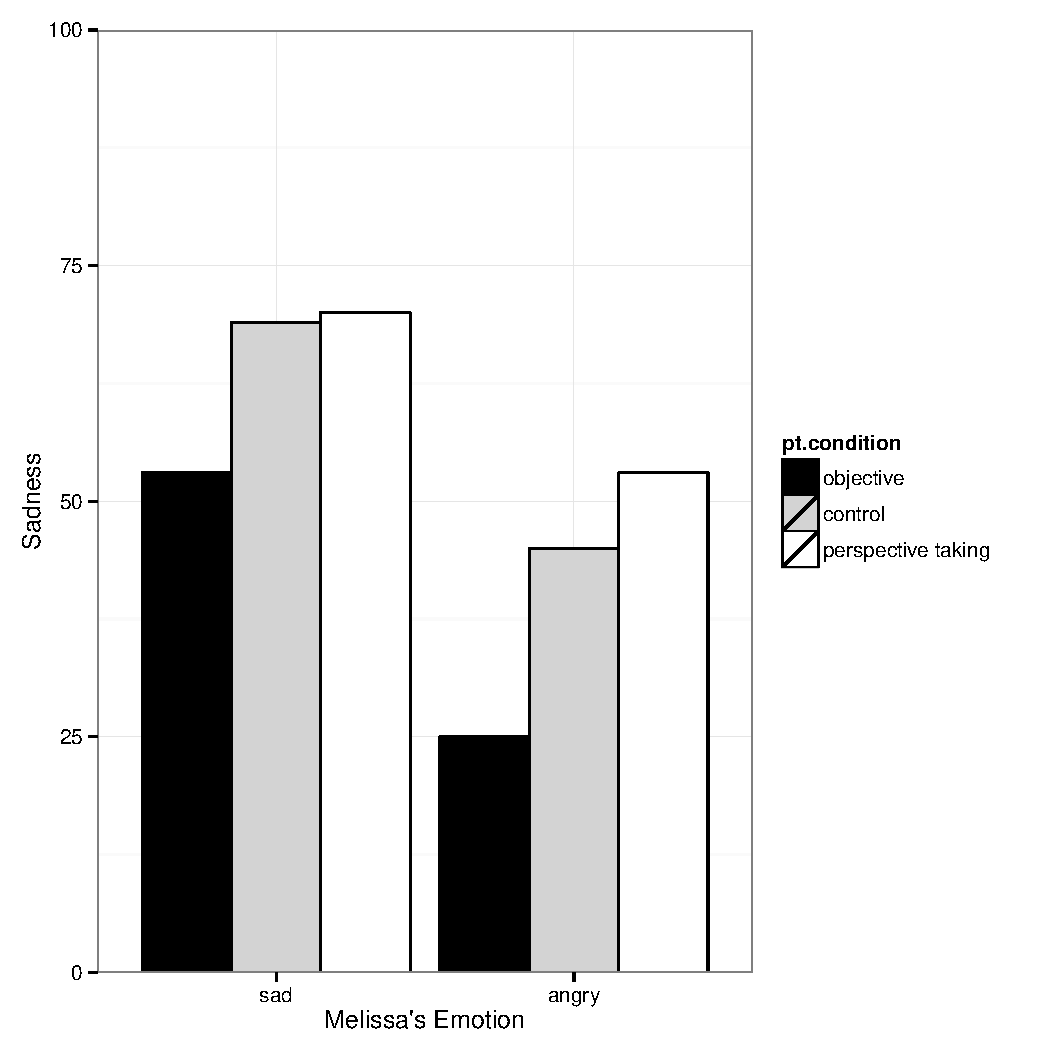
\includegraphics[width=\maxwidth]{figure/Figure1Sad-1} 

\end{knitrout}
\textit{Figure 1. Probability that subjects reported feeling sad by condition.}
\end{figure}


\begin{figure}
\begin{knitrout}
\definecolor{shadecolor}{rgb}{0.969, 0.969, 0.969}\color{fgcolor}
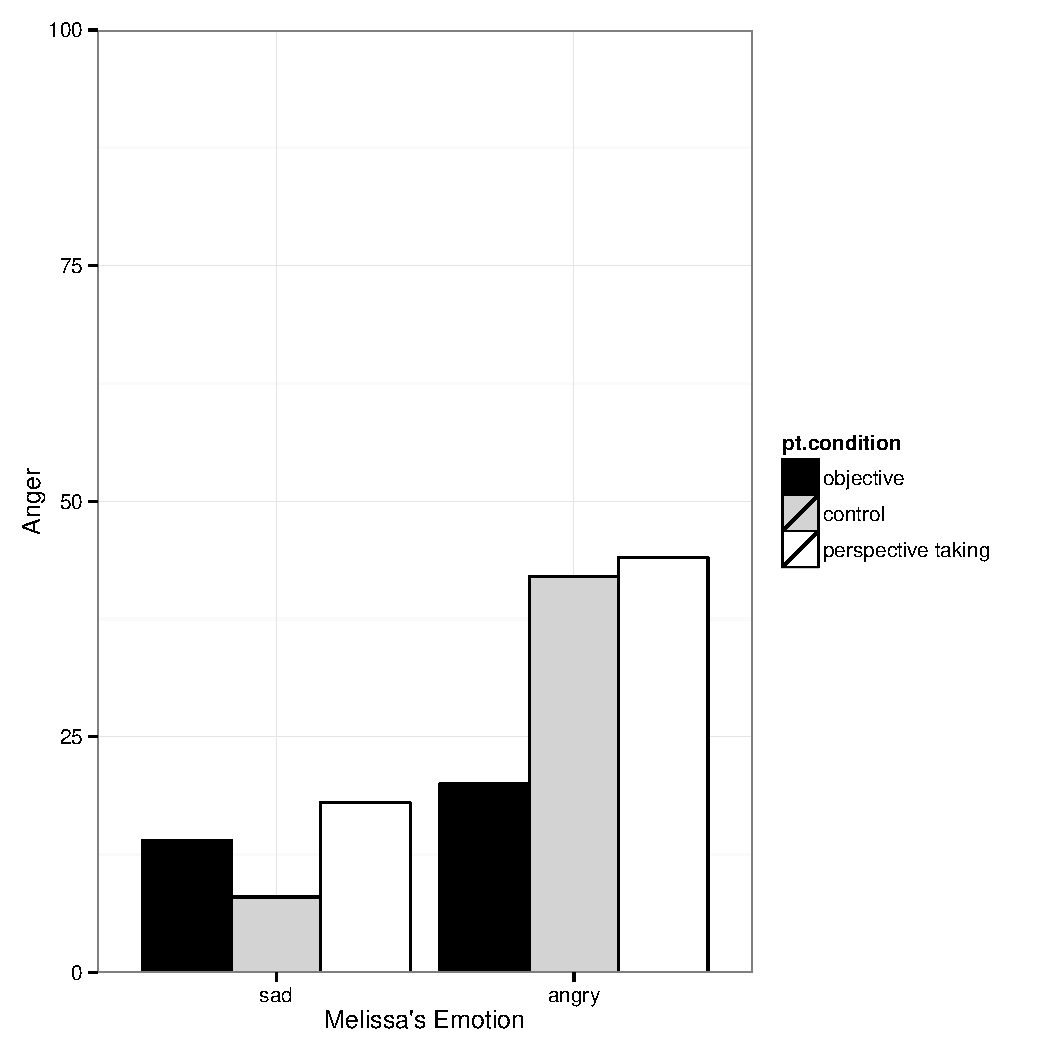
\includegraphics[width=\maxwidth]{figure/Figure2Angry-1} 

\end{knitrout}
\textit{Figure 2. Probability that subjects reported feeling angry by condition.}
\end{figure}



Figure 1 displays the probability that subjects reported feeling sad by condition and Figure 2 displays the probability that subjects reported feeling angry by condition. When Melissa was sad, subjects were just as likely to report feeling sad when they took her perspective (70\%) as when they received no instructions (69\%), \textit{B} = 0.03, \textit{SE} = 0.19, \textit{Z} = 0.14, \textit{p} = 0.88, 95\% CI [\ensuremath{-0.34}, 0.39]. Similarly, when Melissa was angry, subjects were just as likely to report feeling angry when they took her perspective (44\%) as when they received no instructions (42\%), \textit{B} = 0.04, \textit{SE} = 0.17, \textit{Z} = 0.22, \textit{p} = 0.82, 95\% CI [\ensuremath{-0.3}, 0.38]. Overall, there was no evidence that perspective taking made subjects feel how Melissa felt.

\subsubsection{Closed-ended data}

\begin{figure}
\begin{knitrout}
\definecolor{shadecolor}{rgb}{0.969, 0.969, 0.969}\color{fgcolor}
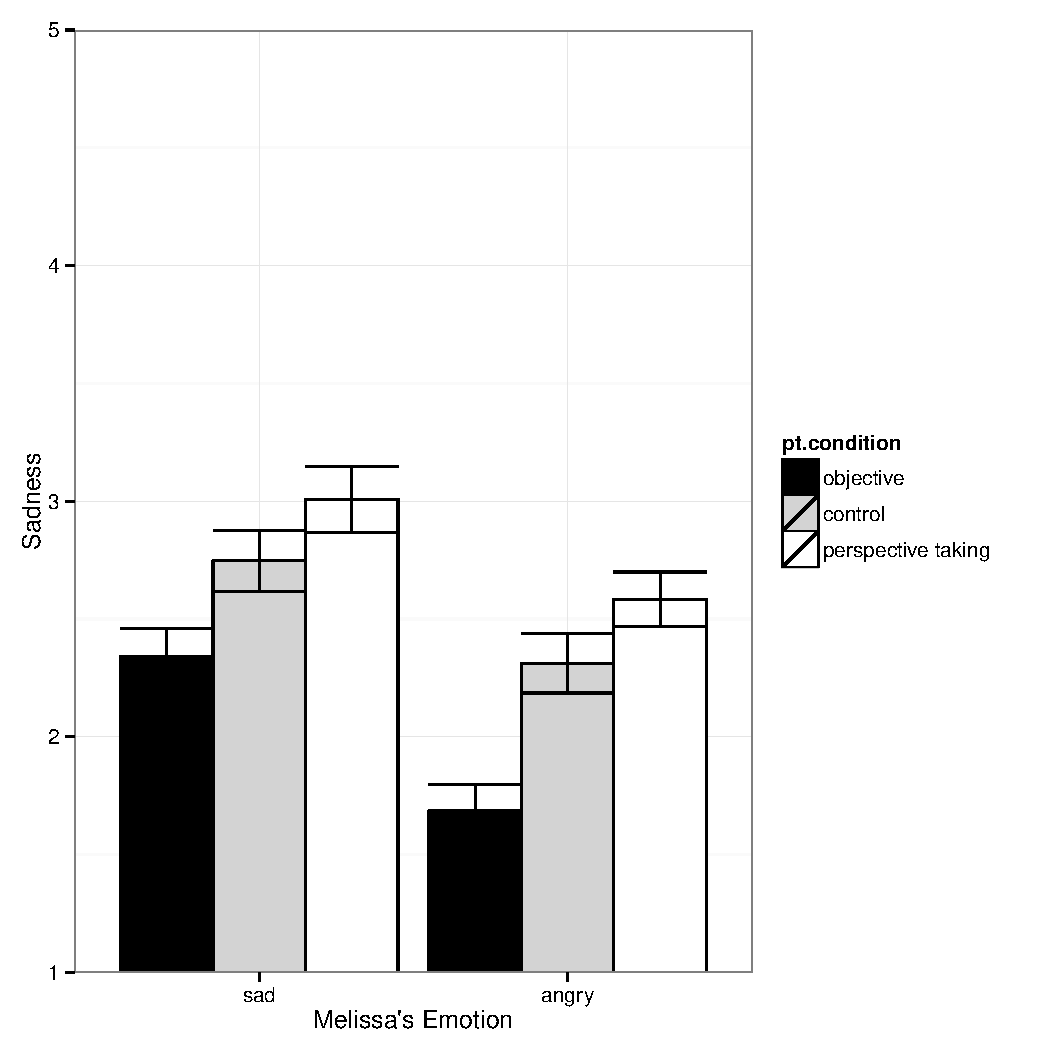
\includegraphics[width=\maxwidth]{figure/Figure3Sad-1} 

\end{knitrout}
\textit{Figure 3. Subjects' average sadness by condition. The bars represent standard errors.}
\end{figure}


\begin{figure}
\begin{knitrout}
\definecolor{shadecolor}{rgb}{0.969, 0.969, 0.969}\color{fgcolor}
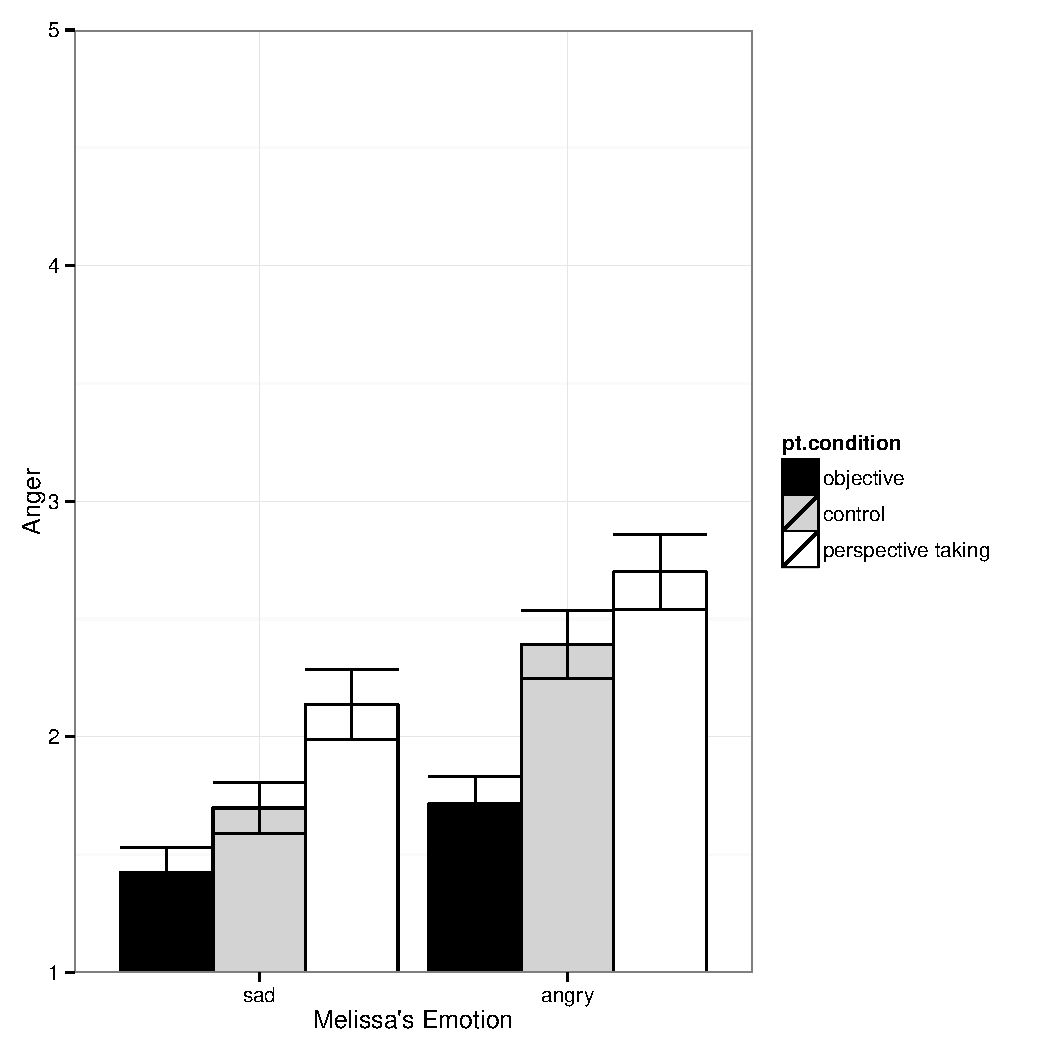
\includegraphics[width=\maxwidth]{figure/Figure4Angry-1} 

\end{knitrout}
\textit{Figure 4. Subjects' average anger by condition. The bars represent standard errors.}
\end{figure}



Figure 3 displays the average sadness that subjects reported feeling by condition and Figure 4 displays the average anger that subjects reported feeling by condition. When Melissa was sad, subjects felt as sad when they took her perspective (\textit{M} = 3.01, \textit{SD} = 1.14) as when they received no instructions (\textit{M} = 2.75, \textit{SD} = 1.1), \textit{B} = 0.13, \textit{SE} = 0.09, \textit{t}(398) = 1.5, \textit{p} = 0.13, 95\% CI [\ensuremath{-0.04}, 0.3]. When Melissa was angry, there was a non-significant trend for subjects to feel angrier when they took her perspective (\textit{M} = 2.7, \textit{SD} = 1.28) than when they received no instructions (\textit{M} = 2.39, \textit{SD} = 1.2), \textit{B} = 0.15, \textit{SE} = 0.09, \textit{t}(396) = 1.66, \textit{p} = 0.098, 95\% CI [\ensuremath{-0.03}, 0.34]. Once again, there was little evidence that perspective taking made subjects feel how Melissa felt.

\subsection{Did Perspective Taking Make Subjects Feel More Sympathetic?}

Aside from feeling how someone else feels, much research has focused on the effects of perspective taking on feeling sympathy, or empathic concern. Although perspective taking didn't seem to make subjects feel what Melissa felt, it might have made them more sympathetic.

\subsubsection{Open-ended data}


When Melissa was sad, subjects were just as likely to report feeling sympathetic when they took her perspective (66\%) as when they received no instructions (68\%), \textit{B} = \ensuremath{-0.04}, \textit{SE} = 0.18, \textit{Z} = \ensuremath{-0.24}, \textit{p} = 0.81, 95\% CI [\ensuremath{-0.4}, 0.31]. Similarly, when Melissa was angry, subjects were just as likely to report feeling angry when they took her perspective (44\%) as when they received no instructions (42\%), \textit{B} = \ensuremath{-0.16}, \textit{SE} = 0.18, \textit{Z} = \ensuremath{-0.91}, \textit{p} = 0.36, 95\% CI [\ensuremath{-0.51}, 0.19]. Overall, there was no evidence that perspective taking made subjects feel sympathetic for Melissa.

\subsubsection{Closed-ended data}



When Melissa was sad, subjects felt as sympathetic when they took her perspective (\textit{M} = 3.69, \textit{SD} = 0.98) as when they received no instructions (\textit{M} = 3.54, \textit{SD} = 1), \textit{B} = 0.08, \textit{SE} = 0.08, \textit{t}(395) = 0.91, \textit{p} = 0.36, 95\% CI [\ensuremath{-0.09}, 0.24]. When Melissa was angry, there was a non-significant trend for subjects to feel more sympathetic when they took her perspective (\textit{M} = 3.76, \textit{SD} = 0.91) than when they received no instructions (\textit{M} = 3.43, \textit{SD} = 1.02), \textit{B} = 0.16, \textit{SE} = 0.08, \textit{t}(395) = 1.93, \textit{p} = 0.054, 95\% CI [\ensuremath{-0.003}, 0.33]. Once again, there was little evidence that perspective taking made subjects feel more sympathy for Melissa.

\subsection{Did Remaining Objective Make Subjects Feel Less Empathy?}

\begin{figure}
\begin{knitrout}
\definecolor{shadecolor}{rgb}{0.969, 0.969, 0.969}\color{fgcolor}
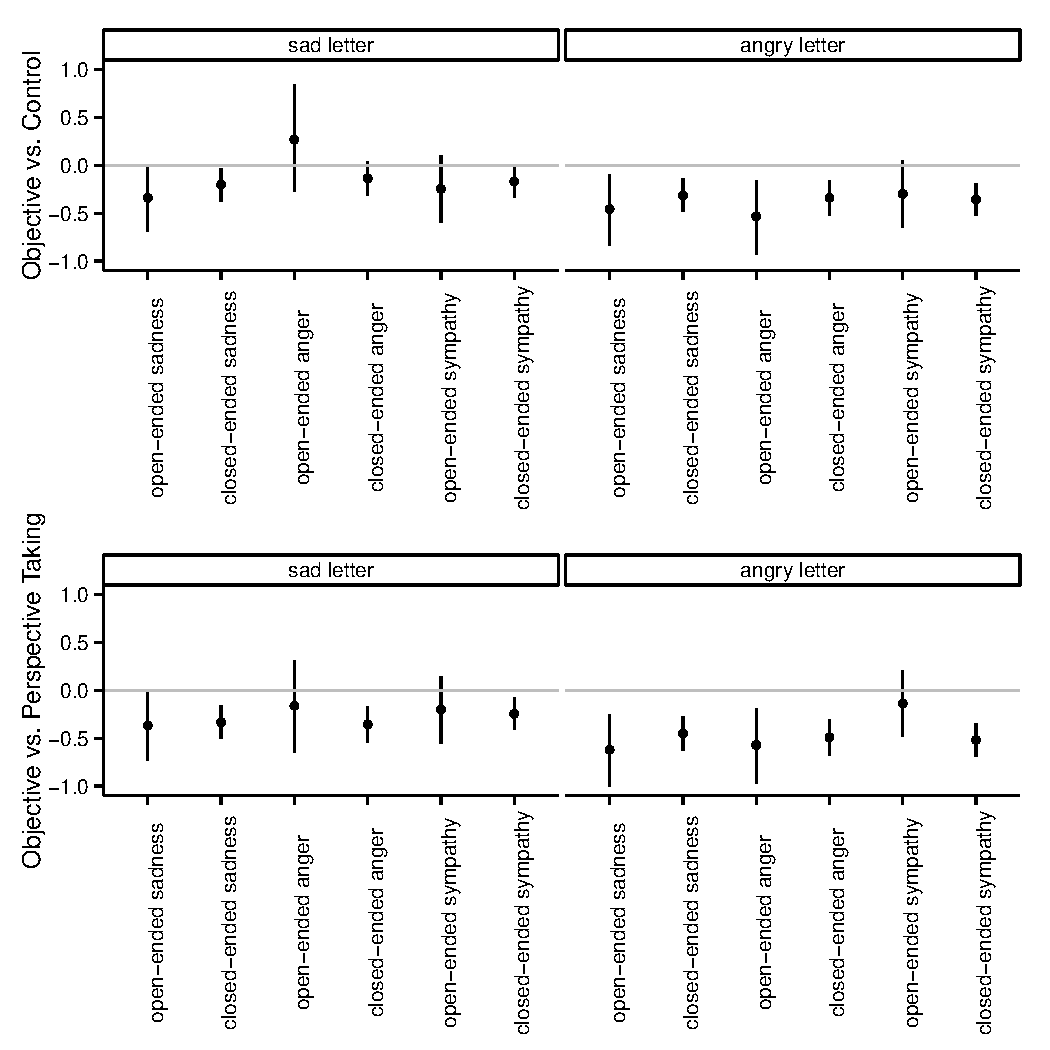
\includegraphics[width=\maxwidth]{figure/Figure5CIPlotsObjectiveVSOthers-1} 
\begin{kframe}\begin{verbatim}
## 
## Call:
## glm(formula = open_sad ~ sad.angry + OvC.sad + PvOC.sad + OvC.angry + 
##     PvOC.angry, family = binomial(link = "logit"), data = ptdata)
## 
## Deviance Residuals: 
##     Min       1Q   Median       3Q      Max  
## -1.5550  -1.2294   0.8421   1.1263   1.6744  
## 
## Coefficients:
##             Estimate Std. Error z value Pr(>|z|)    
## (Intercept)  0.09585    0.10545   0.909   0.3634    
## sad.angry   -0.49634    0.10545  -4.707 2.51e-06 ***
## OvC.sad      0.33971    0.17797   1.909   0.0563 .  
## PvOC.sad     0.13112    0.10695   1.226   0.2202    
## OvC.angry    0.45782    0.18807   2.434   0.0149 *  
## PvOC.angry   0.26093    0.10339   2.524   0.0116 *  
## ---
## Signif. codes:  0 '***' 0.001 '**' 0.01 '*' 0.05 '.' 0.1 ' ' 1
## 
## (Dispersion parameter for binomial family taken to be 1)
## 
##     Null deviance: 558.86  on 403  degrees of freedom
## Residual deviance: 519.58  on 398  degrees of freedom
## AIC: 531.58
## 
## Number of Fisher Scoring iterations: 4
## 
## Call:
## glm(formula = open_sad ~ sad.angry + OvP.sad + CvOP.sad + OvP.angry + 
##     CvOP.angry, family = binomial(link = "logit"), data = ptdata)
## 
## Deviance Residuals: 
##     Min       1Q   Median       3Q      Max  
## -1.5550  -1.2294   0.8421   1.1263   1.6744  
## 
## Coefficients:
##             Estimate Std. Error z value Pr(>|z|)    
## (Intercept)  0.09585    0.10545   0.909  0.36337    
## sad.angry   -0.49634    0.10545  -4.707 2.51e-06 ***
## OvP.sad      0.36653    0.18173   2.017  0.04371 *  
## CvOP.sad     0.10430    0.10482   0.995  0.31974    
## OvP.angry    0.62030    0.18956   3.272  0.00107 ** 
## CvOP.angry   0.09845    0.10247   0.961  0.33671    
## ---
## Signif. codes:  0 '***' 0.001 '**' 0.01 '*' 0.05 '.' 0.1 ' ' 1
## 
## (Dispersion parameter for binomial family taken to be 1)
## 
##     Null deviance: 558.86  on 403  degrees of freedom
## Residual deviance: 519.58  on 398  degrees of freedom
## AIC: 531.58
## 
## Number of Fisher Scoring iterations: 4
## 
## Call:
## lm(formula = sad_mean ~ sad.angry + OvC.sad + PvOC.sad + OvC.angry + 
##     PvOC.angry, data = ptdata)
## 
## Residuals:
##     Min      1Q  Median      3Q     Max 
## -2.0075 -0.6846 -0.1340  0.7535  3.3154 
## 
## Coefficients:
##             Estimate Std. Error t value Pr(>|t|)    
## (Intercept)  2.44573    0.05085  48.097  < 2e-16 ***
## sad.angry   -0.25255    0.05085  -4.967 1.01e-06 ***
## OvC.sad      0.20278    0.08734   2.322 0.020749 *  
## PvOC.sad     0.15459    0.05078   3.044 0.002486 ** 
## OvC.angry    0.31349    0.08829   3.551 0.000430 ***
## PvOC.angry   0.19508    0.05122   3.809 0.000162 ***
## ---
## Signif. codes:  0 '***' 0.001 '**' 0.01 '*' 0.05 '.' 0.1 ' ' 1
## 
## Residual standard error: 1.022 on 398 degrees of freedom
## Multiple R-squared:  0.1414,	Adjusted R-squared:  0.1306 
## F-statistic: 13.11 on 5 and 398 DF,  p-value: 7.882e-12
## 
## Call:
## lm(formula = sad_mean ~ sad.angry + OvP.sad + CvOP.sad + OvP.angry + 
##     CvOP.angry, data = ptdata)
## 
## Residuals:
##     Min      1Q  Median      3Q     Max 
## -2.0075 -0.6846 -0.1340  0.7535  3.3154 
## 
## Coefficients:
##             Estimate Std. Error t value Pr(>|t|)    
## (Intercept)  2.44573    0.05085  48.097  < 2e-16 ***
## sad.angry   -0.25255    0.05085  -4.967 1.01e-06 ***
## OvP.sad      0.33328    0.08859   3.762 0.000194 ***
## CvOP.sad     0.02410    0.05005   0.481 0.630466    
## OvP.angry    0.44936    0.08926   5.034 7.28e-07 ***
## CvOP.angry   0.05921    0.05066   1.169 0.243177    
## ---
## Signif. codes:  0 '***' 0.001 '**' 0.01 '*' 0.05 '.' 0.1 ' ' 1
## 
## Residual standard error: 1.022 on 398 degrees of freedom
## Multiple R-squared:  0.1414,	Adjusted R-squared:  0.1306 
## F-statistic: 13.11 on 5 and 398 DF,  p-value: 7.882e-12
## 
## Call:
## glm(formula = open_sympathy ~ sad.angry + OvC.sad + PvOC.sad + 
##     OvC.angry + PvOC.angry, family = binomial(link = "logit"), 
##     data = ptdata)
## 
## Deviance Residuals: 
##     Min       1Q   Median       3Q      Max  
## -1.5015  -1.2825   0.8849   1.0508   1.1644  
## 
## Coefficients:
##              Estimate Std. Error z value Pr(>|z|)    
## (Intercept)  0.432131   0.102672   4.209 2.57e-05 ***
## sad.angry   -0.110544   0.102672  -1.077   0.2816    
## OvC.sad      0.246042   0.177357   1.387   0.1654    
## PvOC.sad     0.053010   0.104169   0.509   0.6108    
## OvC.angry    0.298919   0.177089   1.688   0.0914 .  
## PvOC.angry  -0.008103   0.101866  -0.080   0.9366    
## ---
## Signif. codes:  0 '***' 0.001 '**' 0.01 '*' 0.05 '.' 0.1 ' ' 1
## 
## (Dispersion parameter for binomial family taken to be 1)
## 
##     Null deviance: 541.62  on 403  degrees of freedom
## Residual deviance: 535.37  on 398  degrees of freedom
## AIC: 547.37
## 
## Number of Fisher Scoring iterations: 4
## 
## Call:
## glm(formula = open_sympathy ~ sad.angry + OvP.sad + CvOP.sad + 
##     OvP.angry + CvOP.angry, family = binomial(link = "logit"), 
##     data = ptdata)
## 
## Deviance Residuals: 
##     Min       1Q   Median       3Q      Max  
## -1.5015  -1.2825   0.8849   1.0508   1.1644  
## 
## Coefficients:
##             Estimate Std. Error z value Pr(>|z|)    
## (Intercept)  0.43213    0.10267   4.209 2.57e-05 ***
## sad.angry   -0.11054    0.10267  -1.077    0.282    
## OvP.sad      0.20254    0.17869   1.133    0.257    
## CvOP.sad     0.09652    0.10341   0.933    0.351    
## OvP.angry    0.13730    0.17577   0.781    0.435    
## CvOP.angry   0.15351    0.10262   1.496    0.135    
## ---
## Signif. codes:  0 '***' 0.001 '**' 0.01 '*' 0.05 '.' 0.1 ' ' 1
## 
## (Dispersion parameter for binomial family taken to be 1)
## 
##     Null deviance: 541.62  on 403  degrees of freedom
## Residual deviance: 535.37  on 398  degrees of freedom
## AIC: 547.37
## 
## Number of Fisher Scoring iterations: 4
## 
## Call:
## lm(formula = symp_mean ~ sad.angry + OvC.sad + PvOC.sad + OvC.angry + 
##     PvOC.angry, data = ptdata)
## 
## Residuals:
##      Min       1Q   Median       3Q      Max 
## -2.68939 -0.69697  0.06522  0.77692  2.27692 
## 
## Coefficients:
##             Estimate Std. Error t value Pr(>|t|)    
## (Intercept)  3.39025    0.04897  69.232  < 2e-16 ***
## sad.angry   -0.08378    0.04897  -1.711   0.0879 .  
## OvC.sad      0.16937    0.08409   2.014   0.0447 *  
## PvOC.sad     0.10768    0.04902   2.197   0.0286 *  
## OvC.angry    0.35585    0.08471   4.201 3.29e-05 ***
## PvOC.angry   0.22754    0.04939   4.607 5.53e-06 ***
## ---
## Signif. codes:  0 '***' 0.001 '**' 0.01 '*' 0.05 '.' 0.1 ' ' 1
## 
## Residual standard error: 0.9802 on 395 degrees of freedom
##   (3 observations deleted due to missingness)
## Multiple R-squared:  0.112,	Adjusted R-squared:  0.1008 
## F-statistic: 9.967 on 5 and 395 DF,  p-value: 5.397e-09
## 
## Call:
## lm(formula = symp_mean ~ sad.angry + OvP.sad + CvOP.sad + OvP.angry + 
##     CvOP.angry, data = ptdata)
## 
## Residuals:
##      Min       1Q   Median       3Q      Max 
## -2.68939 -0.69697  0.06522  0.77692  2.27692 
## 
## Coefficients:
##             Estimate Std. Error t value Pr(>|t|)    
## (Intercept)  3.39025    0.04897  69.232  < 2e-16 ***
## sad.angry   -0.08378    0.04897  -1.711  0.08789 .  
## OvP.sad      0.24621    0.08531   2.886  0.00412 ** 
## CvOP.sad     0.03084    0.04831   0.638  0.52354    
## OvP.angry    0.51923    0.08597   6.040 3.57e-09 ***
## CvOP.angry   0.06416    0.04867   1.318  0.18815    
## ---
## Signif. codes:  0 '***' 0.001 '**' 0.01 '*' 0.05 '.' 0.1 ' ' 1
## 
## Residual standard error: 0.9802 on 395 degrees of freedom
##   (3 observations deleted due to missingness)
## Multiple R-squared:  0.112,	Adjusted R-squared:  0.1008 
## F-statistic: 9.967 on 5 and 395 DF,  p-value: 5.397e-09
## 
## Call:
## glm(formula = open_anger ~ sad.angry + OvC.sad + PvOC.sad + OvC.angry + 
##     PvOC.angry, family = binomial(link = "logit"), data = ptdata)
## 
## Deviance Residuals: 
##     Min       1Q   Median       3Q      Max  
## -1.0759  -0.6681  -0.5415  -0.4202   2.2230  
## 
## Coefficients:
##             Estimate Std. Error z value Pr(>|z|)    
## (Intercept)  -1.2837     0.1322  -9.709  < 2e-16 ***
## sad.angry     0.6332     0.1322   4.789 1.67e-06 ***
## OvC.sad      -0.2684     0.2787  -0.963  0.33553    
## PvOC.sad      0.1973     0.1411   1.398  0.16210    
## OvC.angry     0.5324     0.1973   2.699  0.00696 ** 
## PvOC.angry    0.2034     0.1056   1.926  0.05411 .  
## ---
## Signif. codes:  0 '***' 0.001 '**' 0.01 '*' 0.05 '.' 0.1 ' ' 1
## 
## (Dispersion parameter for binomial family taken to be 1)
## 
##     Null deviance: 447.66  on 403  degrees of freedom
## Residual deviance: 406.16  on 398  degrees of freedom
## AIC: 418.16
## 
## Number of Fisher Scoring iterations: 5
## 
## Call:
## glm(formula = open_anger ~ sad.angry + OvP.sad + CvOP.sad + OvP.angry + 
##     CvOP.angry, family = binomial(link = "logit"), data = ptdata)
## 
## Deviance Residuals: 
##     Min       1Q   Median       3Q      Max  
## -1.0759  -0.6681  -0.5415  -0.4202   2.2230  
## 
## Coefficients:
##             Estimate Std. Error z value Pr(>|z|)    
## (Intercept)  -1.2837     0.1322  -9.709  < 2e-16 ***
## sad.angry     0.6332     0.1322   4.789 1.67e-06 ***
## OvP.sad       0.1617     0.2399   0.674    0.500    
## CvOP.sad     -0.2328     0.1632  -1.427    0.154    
## OvP.angry     0.5713     0.1985   2.878    0.004 ** 
## CvOP.angry    0.1645     0.1048   1.569    0.117    
## ---
## Signif. codes:  0 '***' 0.001 '**' 0.01 '*' 0.05 '.' 0.1 ' ' 1
## 
## (Dispersion parameter for binomial family taken to be 1)
## 
##     Null deviance: 447.66  on 403  degrees of freedom
## Residual deviance: 406.16  on 398  degrees of freedom
## AIC: 418.16
## 
## Number of Fisher Scoring iterations: 5
## 
## Call:
## lm(formula = angry_mean ~ sad.angry + OvC.sad + PvOC.sad + OvC.angry + 
##     PvOC.angry, data = ptdata)
## 
## Residuals:
##     Min      1Q  Median      3Q     Max 
## -1.7000 -0.7154 -0.3913  0.6087  3.3028 
## 
## Coefficients:
##             Estimate Std. Error t value Pr(>|t|)    
## (Intercept)  2.01075    0.05372  37.428  < 2e-16 ***
## sad.angry    0.25815    0.05372   4.805 2.20e-06 ***
## OvC.sad      0.13647    0.09204   1.483 0.138932    
## PvOC.sad     0.19188    0.05378   3.568 0.000404 ***
## OvC.angry    0.33796    0.09304   3.632 0.000318 ***
## PvOC.angry   0.21555    0.05425   3.973 8.42e-05 ***
## ---
## Signif. codes:  0 '***' 0.001 '**' 0.01 '*' 0.05 '.' 0.1 ' ' 1
## 
## Residual standard error: 1.077 on 396 degrees of freedom
##   (2 observations deleted due to missingness)
## Multiple R-squared:  0.1441,	Adjusted R-squared:  0.1333 
## F-statistic: 13.33 on 5 and 396 DF,  p-value: 5.046e-12
## 
## Call:
## lm(formula = angry_mean ~ sad.angry + OvP.sad + CvOP.sad + OvP.angry + 
##     CvOP.angry, data = ptdata)
## 
## Residuals:
##     Min      1Q  Median      3Q     Max 
## -1.7000 -0.7154 -0.3913  0.6087  3.3028 
## 
## Coefficients:
##             Estimate Std. Error t value Pr(>|t|)    
## (Intercept)  2.01075    0.05372  37.428  < 2e-16 ***
## sad.angry    0.25815    0.05372   4.805 2.20e-06 ***
## OvP.sad      0.35606    0.09370   3.800 0.000167 ***
## CvOP.sad    -0.02771    0.05281  -0.525 0.600148    
## OvP.angry    0.49231    0.09442   5.214 2.98e-07 ***
## CvOP.angry   0.06120    0.05345   1.145 0.252869    
## ---
## Signif. codes:  0 '***' 0.001 '**' 0.01 '*' 0.05 '.' 0.1 ' ' 1
## 
## Residual standard error: 1.077 on 396 degrees of freedom
##   (2 observations deleted due to missingness)
## Multiple R-squared:  0.1441,	Adjusted R-squared:  0.1333 
## F-statistic: 13.33 on 5 and 396 DF,  p-value: 5.046e-12
\end{verbatim}
\end{kframe}
\end{knitrout}
\textit{Figure 5. 95\% confidence intervals for the difference in subjects' emotions by condition. Positive values indicate that subjects felt stronger emotions in the control and perspective taking conditions than in the objective condition.}
\end{figure}

There was little evidence that perspective taking made subjects feel how Melissa felt or made them feel sadder or more sympathetic by reducing actor-observer bias. However, remaining objective might have decreased vicarious emotions. Figure 5 displays 95\% confidence intervals for the difference in subjects' emotions between the objective condition and the control and perspective taking conditions. 

When Melissa was sad, subjects were less likely to report feeling sad in the objective condition than in the control and perspective taking conditions, though the comparison between the objective and control conditions in the open-ended data was marginally significant (\textit{p} = .056). Subjects who remained objective also reported feeling less sympathetic than those in the other two conditions in their closed-ended responses. Although the pattern was in the same direction, there were no significant differences in subjects' open-ended reports of sympathy. 

When Melissa was angry, subjects were less likely to report feeling angry int he objective condition than in the control and perspective taking conditions. They also reported feeling less sympathetic than those in the other two conditions in their closed-ended responses, although once again this pattern was not significant in the open-ended emotion reports. 

Although there was some variability in the magnitude of the differences, Figure 5 shows that with only one exception, subjects felt weaker vicarious emotions when they remained objective than in the other two conditions. In contrast there was little evidence that subjects felt stronger vicarious emotions when they took Melissa's perspective than when they received no instructions. 




\section{Discussion}

In this study, remaining objective is what was effortful. It wasn't a neutral control, but active down-regulation. Informally, many subjects described what sounds like common emotion regulation strategies. One said he tried to imagine it was a novel he didn't care about (reappraisal). Another said she imagined looking down from above (self-distancing). Several said it was hard to remain objective, meaning that empathizing required little active effort, but what did require active effort was down-regulating that empathic response. 

Perspective taking is emotional up-regulation and it's only likely to matter when empathizing is hard.


\bibliography{ptreferences}
\bibliographystyle{apacite}

\end{document}
